\documentclass[12pt]{report}
\usepackage[letterpaper,margin=1in]{geometry}
\usepackage[myheadings]{fullpage}
\usepackage{fancyhdr}
\usepackage{graphicx, wrapfig, subcaption, setspace, booktabs}
\usepackage[T1]{fontenc}
\usepackage{fourier}
\usepackage[english]{babel}
\usepackage{sectsty}
\usepackage{verbatim}
\usepackage{listings}
\usepackage{tikz}
\usepackage{tocloft}
\usepackage{xcolor}

% settings for drawing flowchart
\usetikzlibrary{matrix,shapes,arrows,positioning,chains}
\tikzstyle{block} = [rectangle, draw, text centered, rounded corners, minimum height=4em,minimum width=14em]
\tikzstyle{sideblock} = [rectangle, draw, text centered, rounded corners, minimum height=4em, node distance=5.8cm, minimum width=14em]
\tikzstyle{line} = [draw, -latex']

% path for importing images
\graphicspath{{images/}}

% format table of contents
\setlength\cftaftertoctitleskip{0pt}
\onehalfspacing
\setcounter{tocdepth}{2}
\setcounter{secnumdepth}{5}

% format hrule for use in title
\newcommand{\HRule}[1]{\rule{\linewidth}{#1}}

% formatting C++ code
\definecolor{listinggray}{gray}{0.9}
\definecolor{lbcolor}{rgb}{0.9,0.9,0.9}
\lstset{
  backgroundcolor=\color{lbcolor},
  tabsize=4,
  language=C++,
  captionpos=b,
  tabsize=4,
  showstringspaces=false,
  basicstyle=\footnotesize,
  keywordstyle=\color[rgb]{0,0,1},
  stringstyle=\color{red}
}

%-------------------------------------------------------------------------------
% HEADER & FOOTER
%-------------------------------------------------------------------------------
\pagestyle{fancy}
\fancyhf{}
\setlength\headheight{15pt}
\fancyhead[L]{Super Dank Space Adventure}
%\fancyhead[R]{Technical Report}
\fancyfoot[C]{\thepage}

%-------------------------------------------------------------------------------
% TITLE PAGE
%-------------------------------------------------------------------------------

\begin{document}

\title{
        \HRule{0.5pt} \\ [0.5cm]
        \LARGE \textbf{\uppercase{Super Dank Space Adventure}}
        \HRule{0.5pt} \\ [0.5cm]
        \normalsize \textsc{Technical Report} \\}

\date{}

\author{Eric Smith \\
        Erik Juarez \\
        Perry Huynh \\
        Vincente Lara}

\maketitle
\tableofcontents

%-------------------------------------------------------------------------------
% BODY
%-------------------------------------------------------------------------------

% Section title formatting
\sectionfont{\scshape}

\newpage
\section*{1. Requirements}
\addcontentsline{toc}{section}{1. Requirements}

\subsection*{1.1 GitHub}
\addcontentsline{toc}{subsection}{1.1 GitHub}
The project will be contained in a Github repository (Master branch), and the instructor will have the URL and access to view or clone it.

\subsection*{1.2 Source Files}
\addcontentsline{toc}{subsection}{1.1 Source Files}
Each student will have a C++ source file named correctly as described in lab-6. The source file should have a minimum of 500 lines of your own code. Code copy and pasted from a framework does not count as your own code. A header file may also be included.

\subsection*{1.3 Makefile}
\addcontentsline{toc}{subsection}{1.3 Makefile}
The project will have a Makefile that can be used to build your project on the local computers in Room 315. The makefile must compile and link the student files for each student in your group.

\subsection*{1.4 Other}
\addcontentsline{toc}{subsection}{1.4 Other}
For the development of this game, we opted to use the K\&R Indent Style. For our software development process, we used a mix of agile and waterfall. The majority of the functional and nonfunctional requirements are explored in the next section, design.

%-------------------------------------------------------------------------------
% DESIGN
%-------------------------------------------------------------------------------
\newpage
\section*{2. Design}
\addcontentsline{toc}{section}{2. Design}

The design of the game was inspired from games such as Agar.io and Katamari Forever, where the player's goal is to traverse around the area and collide with other objects and gain as much mass as they can. The basic idea of the game is to collide with other objects and gain as much mass as you can, while avoiding larger objects. \bigskip

In order to implement this, we found it best to use and modify the Asteroids framework, to make the game similar to Agar.io, but using X11, OpenGL, and OpenAL in C++. \bigskip

When gaining mass, we decided to take into account the size of the absorbed object, so absorbing something significantly smaller than you would amount to little to no increase in size while absorbing something nearly as big as you would amount to a relatively large increase in size. We also opted to use an inverse exponential function when increasing the player's score and then using the score in a logarithmic function to increase the player's size, rather than simply incrementing by one. We also wanted the size of the enemy objects that are spawned throughout the game to be relative to the player's current size. The size of object would also affect its own velocity. \bigskip

One feature that we definitely needed to implement was a sort of spawn protection, so that as the enemy objects are spawned, they do not spawn directly on top of you and immediately kill you. \bigskip

We wanted to modify the camera, having it so there was a sort of invisible "boundary" around the character, so that when the boundary was passed, the camera would slowly pan towards the direction that the player was moving, simulating a larger area. \bigskip

As for the nonfunctional requirements of the game, we also wanted to add features such as sounds and texture in order to make it look more interesting than using static colors. We also wanted to add the option to restart the game once the player loses, so they would not have to close the program and run it again.

%-------------------------------------------------------------------------------
% IMPLEMENTATION
%-------------------------------------------------------------------------------
\newpage
\section*{3. Implementation}
\addcontentsline{toc}{section}{3. Implementation}

% General
\subsection*{3.1 General}
\addcontentsline{toc}{subsection}{3.1 General}

\subsubsection*{Game States}
The game ran inside a loop within the main and followed the general data flow diagram below: \bigskip

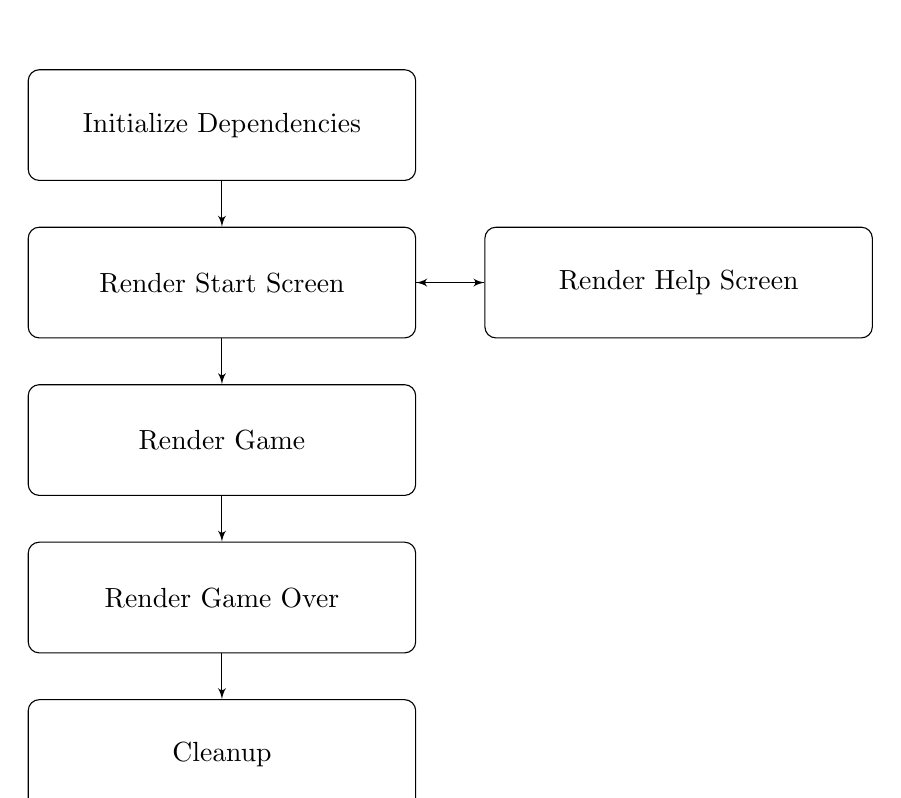
\begin{tikzpicture}[node distance = 2cm, auto]
\node [block] (init) {Initialize Dependencies};
\node [block, below of=init] (start) {Render Start Screen};
\node [sideblock, right of=start] (help) {Render Help Screen};
\node [block, below of=start] (game) {Render Game};
\node [block, below of=game] (gameover) {Render Game Over};
\node [block, below of=gameover] (cleanup) {Cleanup};
\path [line] (init) -- (start);
\path [line] (start) -- (help);
\path [line] (help) -- (start);
\path [line] (start) -- (game);
\path [line] (game) -- (gameover);
\path [line] (gameover) -- (cleanup);
\end{tikzpicture}

\medskip After initializing XWindows, OpenGL, OpenAL, and Textures, the game enters a loop where it it would check for key presses and renders the game's current state. The game initially renders the start screen, which can switch to a Help screen given the Player pressed the 'h' key. After pressing the 'Enter' key to start the game, the loop enters the in-game state and continually calculates and update the positions of every object in the game and renders them. Upon colliding with a larger object, the player is brought to the game over screen. After exiting the program, everything is cleaned up.

\subsubsection*{Restart}
After the game is over, the player has the option to press the 'r' key in order to restart the game without having to close the game and run the program again.

% RENDERING
\newpage
\subsection*{3.2 Rendering}
\addcontentsline{toc}{subsection}{3.2 Rendering}
All rendering was done through various shapes drawn through OpenGL inside a window created by X11. Fonts were rendered using the portion of the framework relating to fonts found in Homework 1 and Lab 2. \bigskip

Player and enemy objects are rendered using OpenGL's \textit{GL\_TRIANGLE\_FAN}. \bigskip

\begin{lstlisting}
glBegin(GL_TRIANGLE_FAN);
float x = (float)g.ship.radius * cos(499 * PI / 180.f);
float y = (float)g.ship.radius * sin(499 * PI / 180.f);

for (int i = 0; i <= 500; i++)
{
	glVertex2f(x, y);
	x = (float)g.ship.radius * cos(i * PI / 180.f);
	y = (float)g.ship.radius * sin(i * PI / 180.f);
}
glEnd();
\end{lstlisting}
\noindent Above is a portion of the code that was used to render the circles before applying textures.

% TEXTURES
\newpage
\subsection*{3.3 Textures}
\addcontentsline{toc}{subsection}{3.3 Textures}
\subsubsection*{Conversion of Images}

Since the game utilizes a wide variety of textures, having a mass amount of \textit{.ppm} files was not very feasible, so it was better to store them as \textit{.png} files and temporarily convert them to \textit{.ppm} files and remove them once we are done with them. Hard coding all of the system commands for conversion and deletion would have been very tedious, inefficient, and inflexible so we used a loop with \textit{<dirent.h>} and iterated through the directory containing the images and converted any files with the \textit{.png} extension and converted them to \textit{*.ppm} files. \bigskip

\begin{lstlisting}
struct dirent *entry;
DIR *dp = opendir("./images/");

if (dp)
{
	while ((entry = readdir(dp)) != NULL)
	{
		if (strstr(entry->d_name, ".png"))
		{
			char t1[256], t2[256];
			char t3[256] = "images/";
			strcpy(t2, entry->d_name);
			int slen = strlen(t2);
			t2[slen - 4] = '\0';
			strcat(t2, ".ppm");
			sprintf(t1, "convert images/%s images/%s", entry->d_name, t2);
			system(t1);
			strcat(t3, t2);
			strcpy(g.imageTemp[g.nt++], t3);
		}
	}
	closedir(dp);
}
\end{lstlisting}
\noindent Above is an a portion of the source code that was used to iterate through the directory and load any \textit{.png} files and convert them to \textit{.ppm} files.

\subsubsection*{Loading the Textures}
The next step in adding textures to the game was to load the converted \textit{.ppm} files and to associate them via OpenGL to their respective objects. The issue with using \textit{<dirent.h>} to load the files was that the order of the files converted was random, so iterating through the array to load certain textures would not work. To solve this issue, the loading of single textures such as the background could be hard coded, but for textures of enemy, we found it was better to utilize a loop and \textit{strcat()} to load the enemy textures, rather than hard code a similar block of code ten times. At the end of the program, we iterate through the array containing the paths for the temporary \textit{.ppm} files and remove them. \bigskip

\begin{lstlisting}
for (int i = 0; i < 6; ++i)
{
	std::stringstream tempStr;
	tempStr<<(i + 1);
	std::string str = tempStr.str();
	char t1[256] = "images/texture_enemy_";
	const char* t2 = str.c_str();
	const char* t3 = ".ppm";
	strcat(t1, t2);
	strcat(t1, t3);

	ppm6CleanupImage(ppm);
	ppm = ppm6GetImage(t1);
}
\end{lstlisting}
\noindent Above is an a portion of the source code that was used to iterate through the directory and load the textures for the enemy objects. \bigskip

\subsubsection*{Rendering the Textures}

The Start Screen, Help Screen, Game Over Screen, and Background were rendered by applying a texture to an area of the screen drawn using \textit{GL\_QUADS}. \bigskip

The textures for the player and enemy objects were rendered by simply applying a texture at the same time the points on the circle are calculated, which produced a "swirl" effect.

% Sounds
\newpage
\subsection*{3.4 Movement}
\addcontentsline{toc}{subsection}{3.4 Movement}
\subsubsection*{Player Movement}
The general implementation for movement in the game was a modified version of the movement function(s) from the Asteroids framework. The player moves towards the location of the mouse cursor on the screen, rather than using the arrow keys. In order to do this we had to add \textit{PointerMotionMask} to the events to check for in the \textit{initXWindows()} function. \bigskip

\begin{lstlisting}
static int savex = 0;
static int savey = 0;

if (savex != e->xbutton.x || savey != e->xbutton.y)
{
	//Mouse moved
	savex = e->xbutton.x;
	savey = e->xbutton.y;

	int y = yres - e->xbutton.y;
	float dx = savex - g.ship.pos[0];
	float dy = y - g.ship.pos[1];
	float len = sqrt(dx * dx + dy * dy);

	g.ship.vel[0] = dx / len;
	g.ship.vel[1] = dy / len;
	normalize(g.ship.vel);
	shipRadiusSpeed();
	normalize(g.ship.vel);
	return;
}
\end{lstlisting}

\noindent Above is a portion of the source code that was used to have the player move towards the location of the mouse cursor. \bigskip

\subsubsection*{Velocity}
The speed of an object (player or asteroid) is dependent on the radius of the object. First we initialize each object with a random vector speed. We came up with a math function that took the radius and scaled it down to an appropriate speed (decreasing speed as the radius grows larger).\bigskip
\begin{lstlisting}
Flt radiusVel = ( ( 500.0 / ( g.ship.radius + 100.0 ) ) - 2.0 )
\end{lstlisting}

\medskip
The first problem encountered with the velocity is that the speed is calculated by adding the squares of the \textit{x} and \textit{y} coordinates of the vector. We take the ratio of the \textit{x} and \textit{y} coordinates of the vector and compare them to the magnitude of that speed. The ratio of the coordinate to the total speed is the same regardless of what you scale it up or down to. We then multiply the ratio of \textit{x-to-speed} and \textit{y-to-speed} by the calculated radius velocity and we get the result of the same directional movement with a properly scaled speed. \bigskip

\begin{lstlisting}
Flt radiusVel = ( ( 500.0 / ( g.ship.radius + 100.0 ) ) - 2.0 );

if ( radiusVel < 0 )
{
	radiusVel = 0.01;
}

Flt xVel = g.ship.vel[0];
Flt yVel = g.ship.vel[1];
Flt speed = sqrt( ( xVel * xVel ) + ( yVel * yVel ) );
Flt xRatio = ( xVel / speed ) * radiusVel;
Flt yRatio = ( yVel / speed ) * radiusVel;

g.ship.vel[0] = xRatio;
g.ship.vel[1] = yRatio;
\end{lstlisting}

\noindent Above is an a portion of the source code that was used to calculate the player's current velocity.

% Growth
\newpage
\subsection*{3.5 Growth}
\addcontentsline{toc}{subsection}{3.5 Growth}
For the player's growth, we decided to use an inverse logarithmic function when increasing the player's score, in order to have it so absorbing a small object amount to little gain in size, and absorbing an object relatively close to the player's size results in a high gain in size. \bigskip

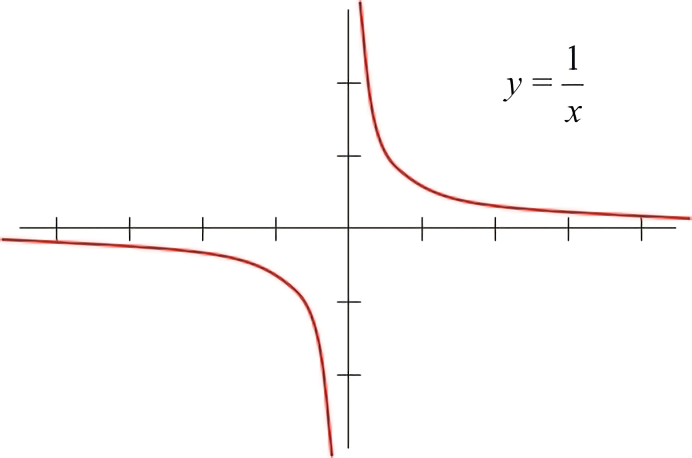
\includegraphics[width=\textwidth]{inverse_log_graph}

\medskip \noindent The graph is a relatively close representation of the mathematical principle of an inverse relationship between the differential of radius to growth in radius.

% Camera
\newpage
\subsection*{3.6 Camera}
\addcontentsline{toc}{subsection}{3.6 Camera}
Our idea for camera implementation was inspired by the presentation of a game during class. Our first thought was to change the position of the player while having the camera follow them. This ended up being more difficult than we anticipated. we decided to implemented a camera that had the world move around our character. \bigskip

When our players velocity changes, we subtract that velocity from the objects within our world. This creates the illusion that our players character is moving throughout the world. To make it more apparent that our player is moving, we implemented a dead zone in the middle of the screen. \bigskip

When the player is within a certain box in the middle of the screen, the camera is static and the player is changing position on the screen. When the player reaches the edges of the box, the camera shifts from static to dynamic and follows the character around the world. To do this, we created boundaries within the world. \bigskip

If the player's position is within these boundaries, then we change the position of the ship. If the player's position is outside of these boundaries, then we keep the players position constant and change the position of the asteroids.

% Camera
\newpage
\subsection*{3.7 Spawning of Enemy Objects}
\addcontentsline{toc}{subsection}{3.7 Spawning of Enemy Objects}
All of the enemy objects were created as nodes in a linked list, each initialized with a random radius that is scaled to be challenging, but not impossible. The random radius is calculated through a random number generator and scaled with the player's current radius and constants that give it a range of values that give the player slightly more asteroids smaller than them, but still enough large ones that need avoiding. Prior to adding the textures, the asteroids were colored depending on their size compared to the player, but after adding the textures, the player has to decide whether the asteroid is small enough to eat, or a game ender. \bigskip

\begin{lstlisting}
Asteroid *a = new Asteroid;
a->nverts = 8;
a->radius = (rnd() * 2.0 * g.ship.radius) - (rnd() * 0.5 * g.ship.radius);
a->textureId = rand() % 6;
\end{lstlisting}

\noindent Above is a portion of the code used when adding an enemy object. The object is initialized with a size relative to the player's current size, and given a random texture value.

% Spawn Protection
\newpage
\subsection*{3.8 Spawn Protection}
\addcontentsline{toc}{subsection}{3.8 Spawn Protection}
In order to provide some protections to the player, we came up with idea of having an "invisible box" around the player that prevents other objects from spawning inside, making it so a large object cannot simply spawn right on top of the player immediately causing them to lose the game. \bigskip

\begin{lstlisting}
Flt tmpx = xres >> 2;
Flt tmpy = yres >> 2;

if ( a->pos[0] <= ( 3.0 * tmpx ) &&
	a->pos[0] >= tmpx &&
	a->pos[1] <= ( 3.0 * tmpy ) &&
	a->pos[1] >= tmpy)
{
	if ((a->pos[0] <= (2.0 * tmpx)) && (a->pos[0] > tmpx))
	{
		a->pos[0] -= 1.25 * tmpx;
		a->pos[2] = 0.0f;
	}
	else
	{
		a->pos[0] += 1.25 * tmpx;
		a->pos[2] = 0.0f;
	}
}
\end{lstlisting}
\noindent Above is a portion of the source code used in adding another object to check whether the object will be within the boundary around the player, and if it is move it.

% Sounds
\newpage
\subsection*{3.9 Sounds}
\addcontentsline{toc}{subsection}{3.9 Sounds}
We were initially planned and used the FMOD library for the playback of the sounds of our game. However we found out that the library was was not free and open source, so the professor would not accept it as a valid library to play sounds in the game. Since this was the case we had to switch to a free and open source library, so we decided to use OpenAL. We had already begun using FMOD for our game's sound so we had to migrate everything to OpenAL as soon as possible since it was a couple days until the project was due. The sounds for the game were then re implemented using OpenAL and the OpenAL Utility Toolkit. \bigskip

The sounds for the game came from Nintendo's Kirby series. The various sounds play when a certain action in the game screen occurs like a collision with another object (when you devour another planet) and there are many other sounds that loop while there is an action being executed i.e. during the start screen, game over screen, play screen, etc.) \bigskip

The way OpenAL works is very similar to OpenGL but instead of working with graphics you work with sound. In order to be able to play sounds you must first initialize the audio devices and set the position, orientation, gain, and many other factors in consideration to the listener. \bigskip

\begin{lstlisting}
float vec[6] = {0.0f,0.0f,1.0f, 0.0f,1.0f,0.0f};
alListener3f(AL_POSITION, 0.0f, 0.0f, 0.0f);
alListenerfv(AL_ORIENTATION, vec);
alListenerf(AL_GAIN, 1.0f);
\end{lstlisting}

\medskip This is due to the fact that OpenAL supports multichannel audio for a 7.1 surround sound output. After that there must be an ALuint source and buffer. Then a buffer is created from an audio file (OpenAL supports many types) and then the buffer is assigned to a source. The source then has many parameters which can be adjusted including but not limited to volume, pitch, and looping. \bigskip

\begin{lstlisting}
alSourcef(alSource, AL_GAIN, 1.0f);
alSourcef(alSource, AL_PITCH, 1.0f);
alSourcei(alSource, AL_LOOPING, AL_FALSE);
\end{lstlisting}

\medskip After finishing using all the sounds just like OpenGL one must clear all the objects created by the program which includes deleting all the sources, all the buffers, and finally closing all the devices currently active. \bigskip

One of the main problems encountered with the sounds was the fact that if we wanted to play a sound in an event which took place inside a loop i.e. the start screen then the sound would not be played but instead a rather repetition of the first part of the sound would play (the sound was being played over and over at the beginning of the loop). 

\begin{lstlisting}
bool gameplay = false;

if (gameplay == false)
{
	stop_playing(alSource);
	alSourcePlay(alSource1);
	gameplay = true;
}
\end{lstlisting}

The solution for this was not as elegant as we hoped but it worked it consisted of creating a boolean value and then setting it to true after playing it. While there were many other challenges this one was the one that was most challenging due to the fact that it was so simple we wanted to make it complicated. \bigskip

Overall sounds using OpenAL was a great experience and while there are many improvements both in efficiency and style which can be done to our code. Being the first time using it is absolutely awesome. 


% Score
\newpage
\subsection*{3.10 Score}
\addcontentsline{toc}{subsection}{3.10 Score}
The player's score is based on the amount of mass they have gained since the game started. The score is equivalent to the player object's current radius, which increases relative to the size of the object they absorb. The score is rendered on the screen using the portion of the framework relating to fonts found in Homework 1 and Lab 2, using \textit{fonts.h} and \textit{libggfonts.a} \bigskip

%-------------------------------------------------------------------------------
% TESTING
%-------------------------------------------------------------------------------
\newpage
\section*{4. Testing}
\addcontentsline{toc}{section}{4. Testing}

The methods of testing utilized in the project included both white-box and black-box testing. For white-box testing, the area being tested was usually delegated to the contributor to that portion of the code, unless they requested help from others as each group member mainly focused on their portion, rather than extensively learn about all aspects of each others' code. Black-box testing was generally done by all members of the group. A majority of the debugging was done through print statements scattered throughout sections of a code to see where an issue might be occurring. We were attempting to determine whether our functions were receiving the proper values of variables and if they were being affected in unintentional ways. Another reason for these output statements was to get hard data from the game objects so we could use that data to assist in our scaling to make the game grow and progress in a smooth manner. \bigskip

A practice that greatly helped our group throughout the coding and testing process was pair programming. Having another set of eyes parse through the code while the main developer was coding was extremely helpful in spotting any issues that arose during coding and debugging. \bigskip

Testing was also done by compiling and running the game on various different computers and Linux distributions, such as Ubuntu and Arch Linux. Some issues arose when accessing the OpenAL library files with some of the Linux distributions we tested because they resided in a different directory, so the \textit{Makefile} had to altered to successfully compile. We also found an interesting bugs with certain Linux distrubutions such as Ubuntu, where using the the computer's function keys to change the volume would result in a segfault. Another bug that took us a long time to find was the growth of the player upon absorbing another object. We 

%-------------------------------------------------------------------------------
% DELIVERY/MAINTENANCE
%-------------------------------------------------------------------------------
\newpage
\section*{5. Delivery/Maintenance}
\addcontentsline{toc}{section}{5. Delivery/Maintenance}
Our group decided on using one combined presentation, with each group member talking about their respective contribution to the project. Each member provided a separate document containing their phase of the technical report and contribution for the implementation section, where it was then combined and formatted using LaTeX. Maintenance was not in mind for this game as it was a project for a class so future features would not be implemented and bugs that may arise would not be fixed unless someone wanted to continually work on the game.

%-------------------------------------------------------------------------------
% SCREENSHOTS
%-------------------------------------------------------------------------------
\newpage
\section*{6. Screenshots}
\addcontentsline{toc}{section}{6. Screenshots}

\subsection*{6.1 Start Screen}
\addcontentsline{toc}{subsection}{6.1 Start Screen}
\includegraphics[width=\textwidth]{start_screen}

\subsection*{6.2 Help Screen}
\addcontentsline{toc}{subsection}{6.2 Help Screen}
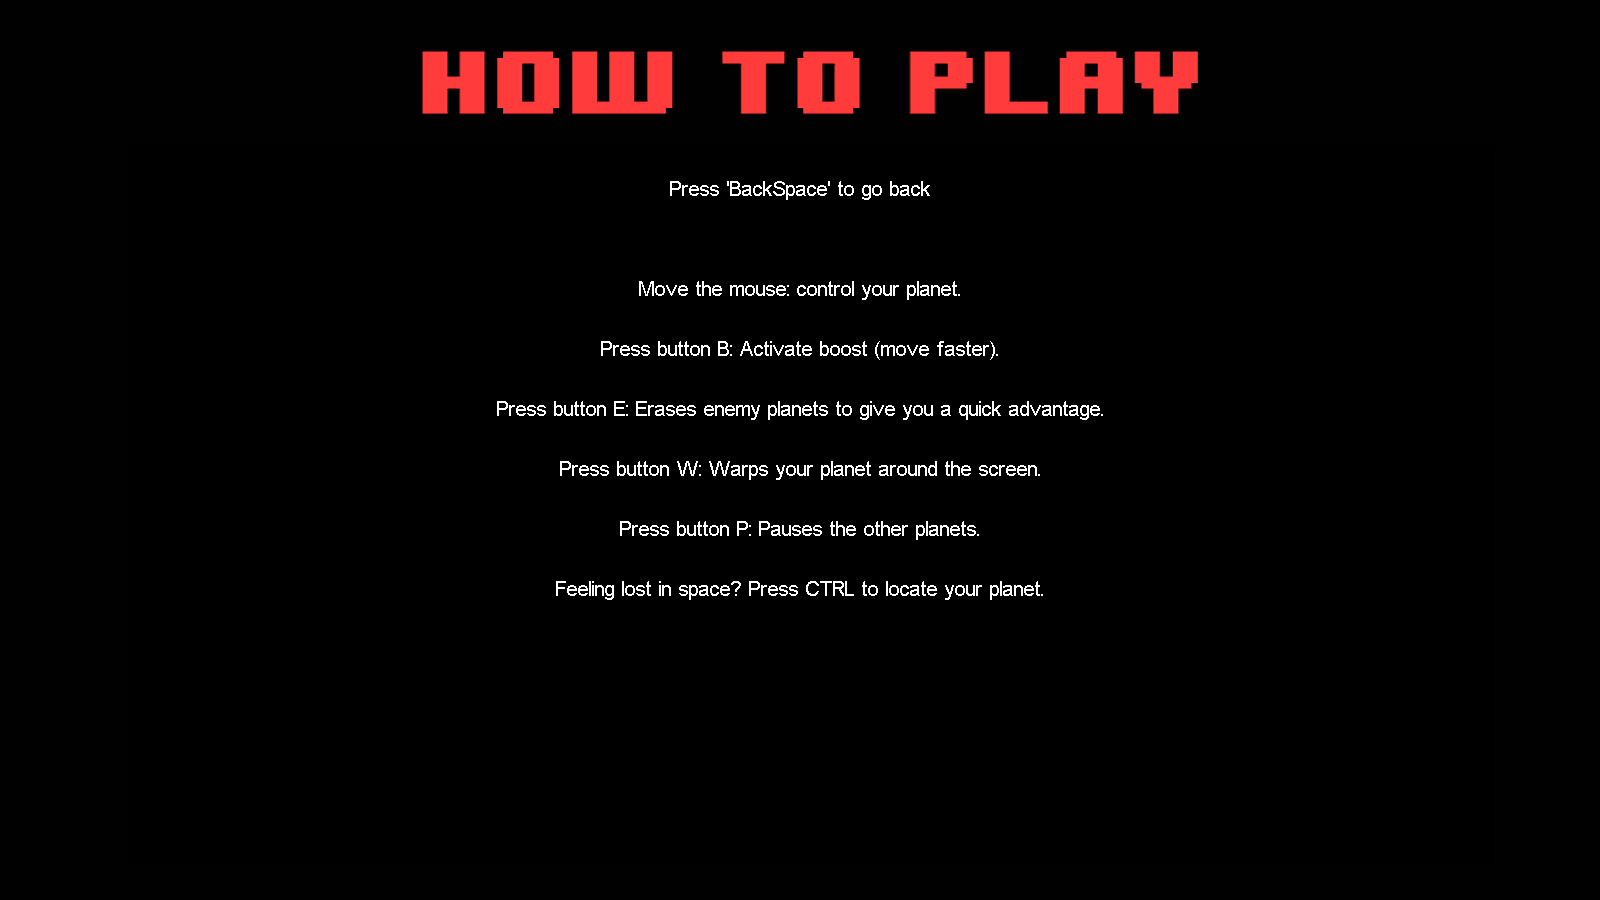
\includegraphics[width=\textwidth]{help_screen}

\subsection*{6.3 Main Game Screen}
\addcontentsline{toc}{subsection}{6.3 Main Game Screen}
\includegraphics[width=\textwidth]{main_game}

\subsection*{6.4 Game Over Screen}
\addcontentsline{toc}{subsection}{6.4 Game Over Screen}
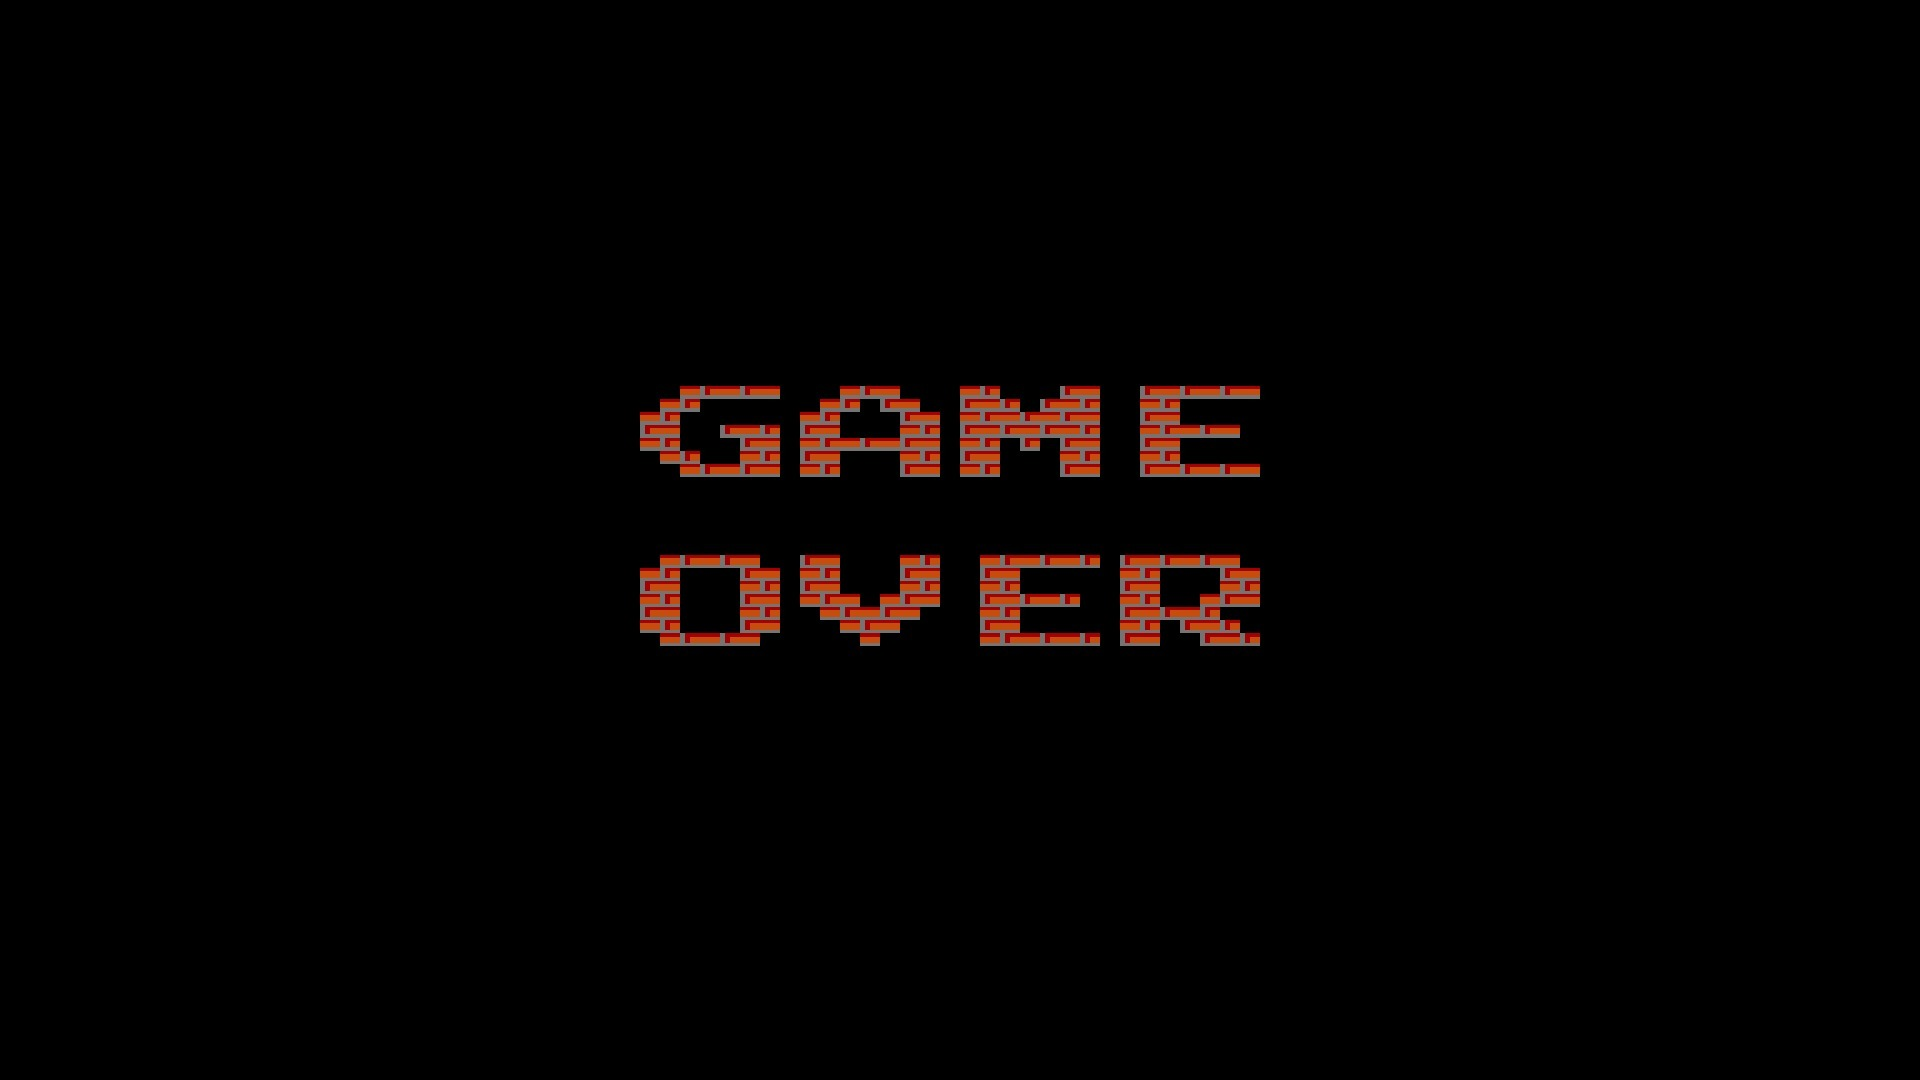
\includegraphics[width=\textwidth]{screen_gameover}

\end{document}
